\documentclass[handout]{beamer}
\usepackage[T1]{fontenc}
\usepackage[utf8]{inputenc}
\usepackage{lmodern}
\usepackage[english]{babel}
\usepackage{tikz}
\usetheme{Warsaw}
%\usefonttheme{serif}

\title[\textsc{Fabrication and measurements of NIS junctions}]{\textsc{Fabrication and measurements of\\NIS junctions to characterize\\plasma etching}}
\author{\textsc{Nicolas Paillet}}
\institute{Aalto University}
\date{11 August 2015}

\setbeamersize{text margin left=0.5cm,text margin right=0.5cm}

\begin{document}
    \begin{frame}
        \titlepage
    \end{frame}

    
    \begin{frame}
        \frametitle{\textsc{The nanowires project}}
        \framesubtitle{Introduction}
        Two types of InAs Nanowires coming from Copenhaguen :
        
        \begin{itemize}
            \item[$\bullet$]{Without barrier, and covered with Al}
            \item[$\bullet$]{With InGaAs barrier, without Al} 
        \end{itemize}
         
        For the covered ones :
        \begin{itemize}        
        \item[$\longrightarrow$] {Al heavily oxidized by the travel}
        \item[$\longrightarrow$] {Get rid of this oxide by Plasma Etching}
        \item[$\longrightarrow$] {Fabrication of NIS structures to characterize the Plasma}
        \end{itemize}
    \end{frame}

    \begin{frame}
        \frametitle{\textsc{Experimental Protocol}}
        \framesubtitle{Parameters}
    
        \begin{itemize}
            \item{4 Pads pattern}
         \end{itemize}   
     
        \centering
        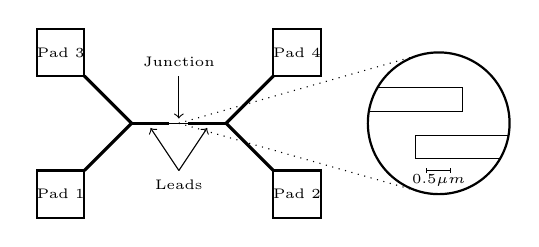
\begin{tikzpicture}[scale=0.6]
                    \draw [thick](0,0)--++(1,0)--++(0,1)--++(-1,0)--cycle;
                    \draw [thick](0,3)--++(1,0)--++(0,1)--++(-1,0)--cycle;
                    \draw [thick](5,0)--++(1,0)--++(0,1)--++(-1,0)--cycle;
                    \draw [thick](5,3)--++(1,0)--++(0,1)--++(-1,0)--cycle;
                    \draw [very thick](1,1)--(2,2);
                    \draw [very thick](1,3)--(2,2);
                    \draw [very thick](5,1)--(4,2);
                    \draw [very thick](5,3)--(4,2);
                    \draw [very thick](2,2)--(2.8,2);
                    \draw [very thick](4,2)--(3.2,2);
                    \draw (2.8,2)--(3.2,2);
                    \draw [->] (3,3)--(3,2.1);
                    \draw (3,3)node[above]{\tiny{Junction}};
                    \draw (0.5,0.5)node{\tiny{Pad 1}};
                    \draw (0.5,3.5) node{\tiny{Pad 3}};
                    \draw (5.5,0.5)node{\tiny{Pad 2}};
                    \draw (5.5,3.5)node{\tiny{Pad 4}};
                    \draw [->] (3,1)--(2.4,1.9);
                    \draw [->] (3,1)--(3.6,1.9);
                    \draw (3,1)node[below]{\tiny{Leads}};
                    \draw [dotted,thin] (3,2)--(8.1,3.45);
                    \draw [dotted,thin] (3,2)--(8.1,0.55);
                    \draw [thick](8.5,2) circle(1.5);
                    \draw (7.2,2.75)--(9,2.75)--(9,2.25)--(7.02,2.25);
                    \draw (9.8,1.25)--(8,1.25)--(8,1.75)--(9.98,1.75);
                    \draw (8.25,1.05)--(8.25,0.95);
                    \draw (8.75,1.05)--(8.75,0.95);
                    \draw (8.25,1)--(8.75,1);
                    \draw (8.5,0.8)node{\tiny{0.5$\mu m$}};
            \end{tikzpicture}
            
            \begin{itemize}
                \item{4x5 matrix with 4 Surface areas : 0.5, 1, 1.5 \& 2 $\mu m^2$}
                \item{5 EBL doses, from 2000 to 3000 by 250 $c/\mu m^2$}
                \item{Development 20s MIBK, 20s Methyglycol, IPA}
                \item{Al 20nm, Cu 25nm}
                \item{Optionnal : Oxidation and Plasma (Pressure$=10^{-4}mbar$, Power$=40mA$, Extraction$=-0.8kV$, then $0.25kV$, Ion Energy$=1.5kV$)} 
                \item{4 probe measurements with a probestation}
            \end{itemize}  
                
    \end{frame}

    \begin{frame}
        \frametitle{\textsc{Reference samples}}
        \framesubtitle{Room temperature measurements}
        
        \begin{columns}[onlytextwidth]
            \begin{column}{0.5\textwidth}
            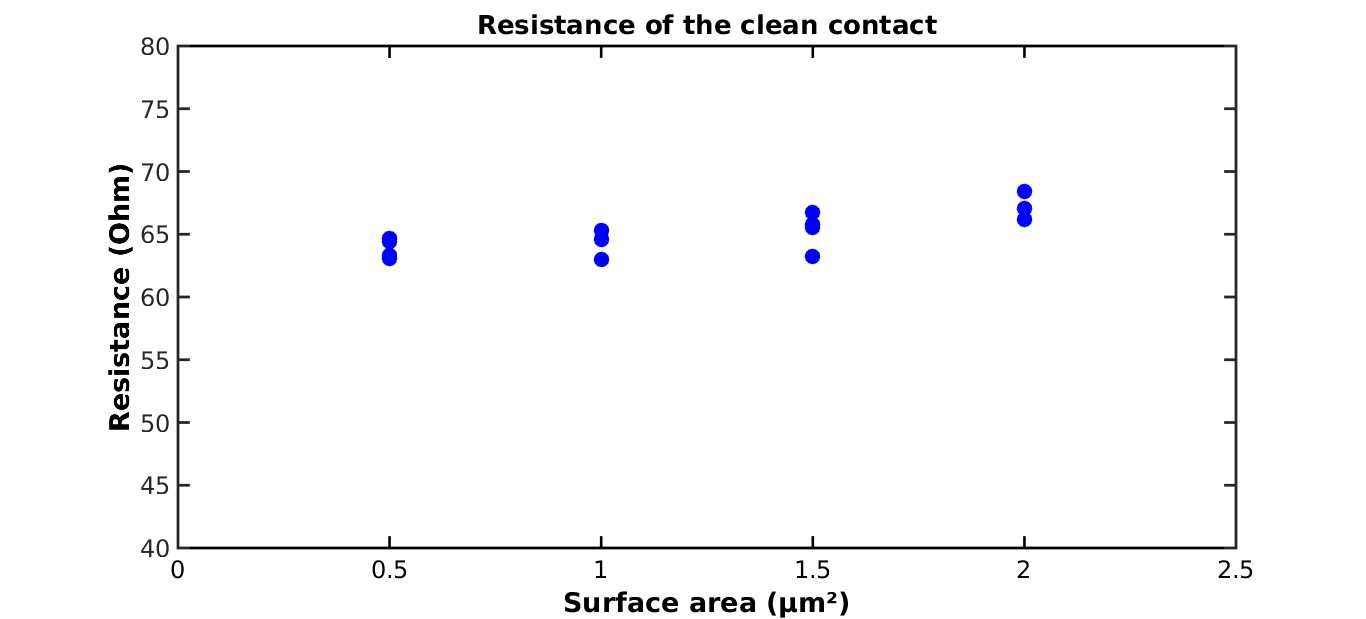
\includegraphics[width=150pt]{Rclean.png}\\
                     
            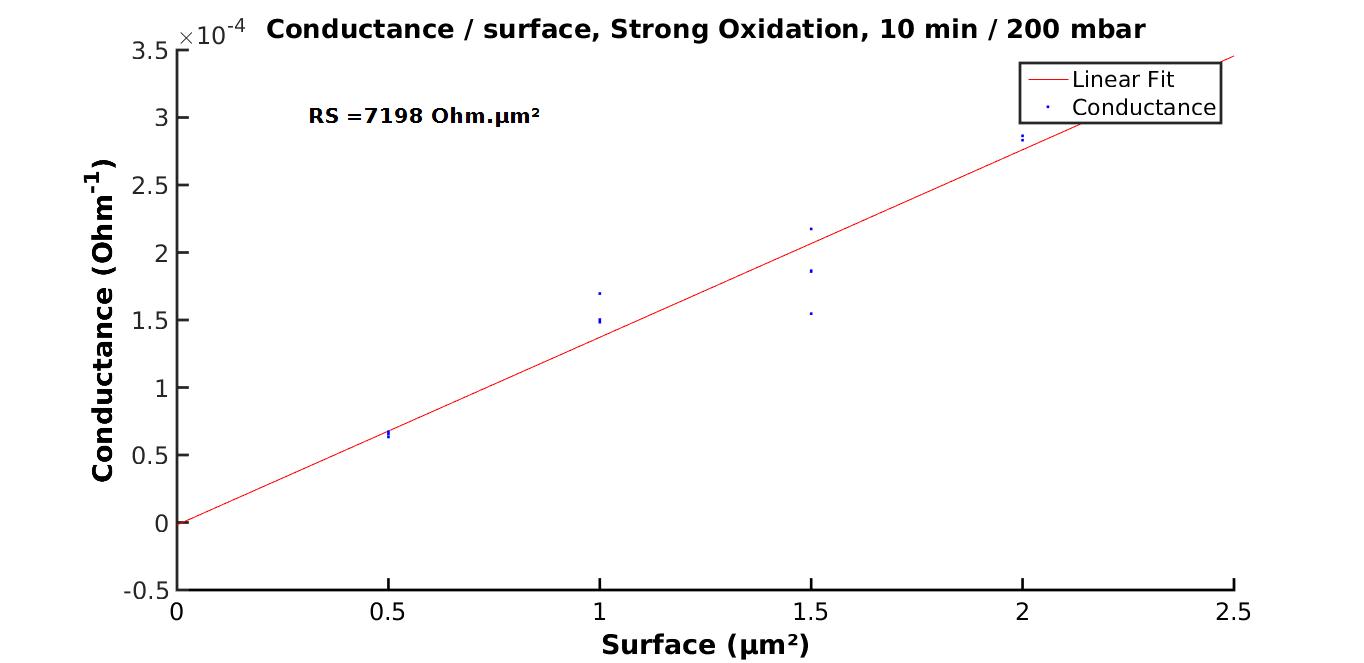
\includegraphics[width=150pt]{ConductanceFitStrongOx.png}\\
                       
            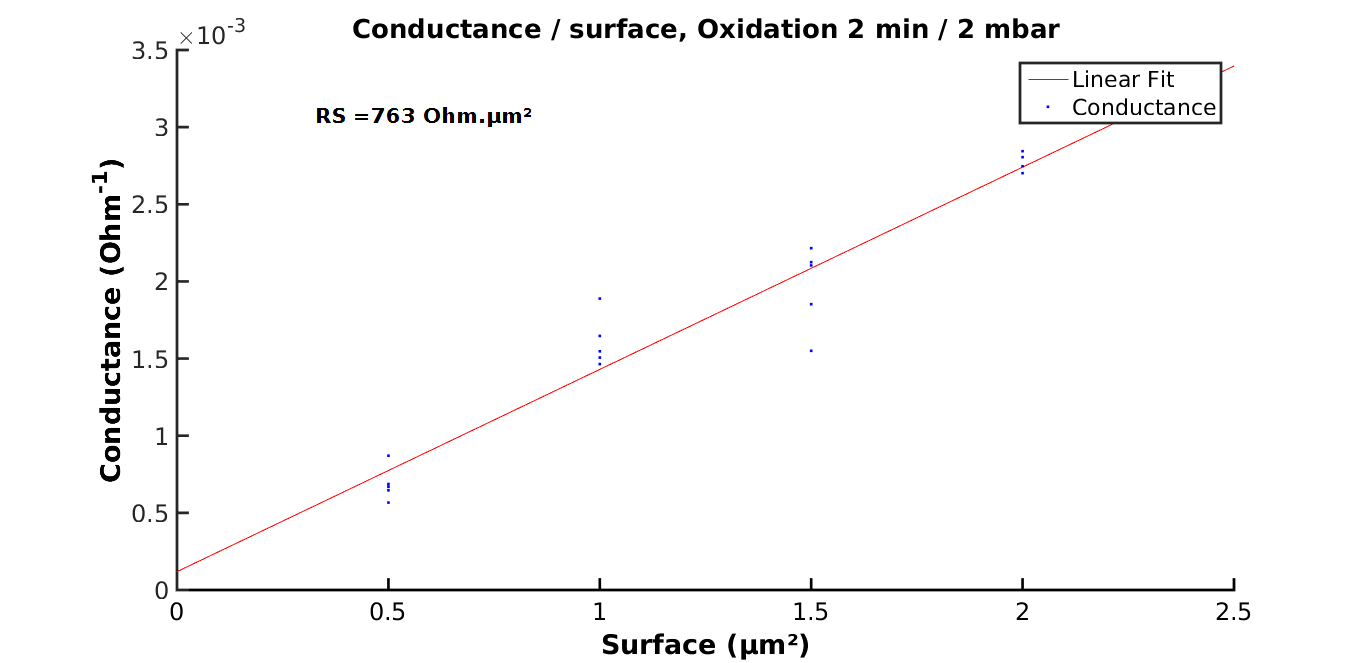
\includegraphics[width=150pt]{ConductanceFitOx.png}
            \end{column}
            
            \begin{column}{0.5\textwidth}
            
            $\bullet$  Clean Contact Al + Cu\\without Plasma\\
            \[R=\sum_{Cu,Al}\dfrac{\rho l}{S}\simeq 78 \Omega\]
            \vspace{0.1cm}
            
            $\bullet$  Strong Oxidation reference\\10min / 200mbar without Plasma\\
            \[RS=7198 \Omega.\mu m^2\]
            \vspace{0.1cm}
            
            $\bullet$  Regular Oxidation reference\\2min / 2mbar without Plasma\\
            \[RS=763 \Omega.\mu m^2\]
            \end{column}
            
        \end{columns}
        
    \end{frame}
    
    \begin{frame}[allowframebreaks]
        \frametitle{\textsc{Plasma Tests}}
        \framesubtitle{Room temperature measurements}
        
        $\bullet$  Position of the sample, Plasma Etching 10 min, before Oxigen cleaning
        \vspace{0.3cm}
               
        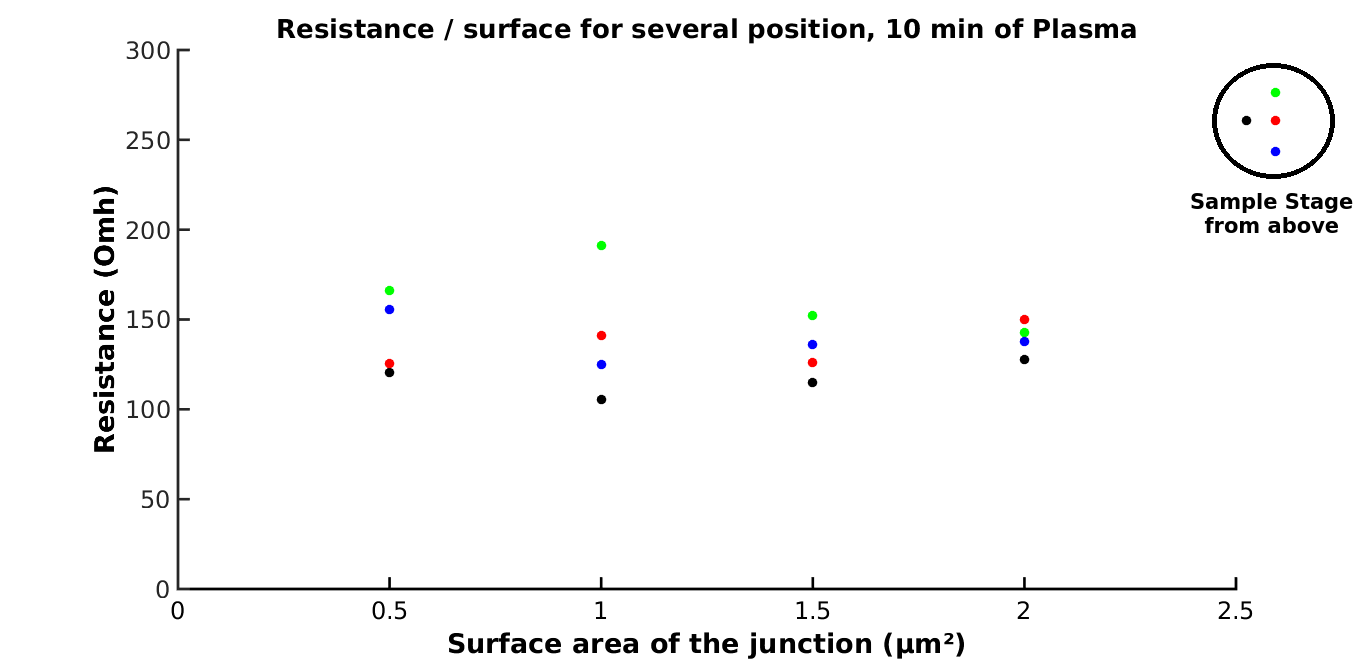
\includegraphics[width=330pt]{R_Position.png}\\
        $\Rightarrow$ Plasma is homogeneous \& 10 min seems enough to etch the oxide : no surface dependance and same order of magnitude as clean contact.
        \vspace{0.5cm}
        
        $\bullet$ Duration of the Plasma Etching
        \vspace{0.3cm}
        
        \begin{columns}[onlytextwidth]
            \begin{column}{0.5\textwidth}
                \hspace{0.5cm} $\bullet$ Before Oxigen cleaning\\
                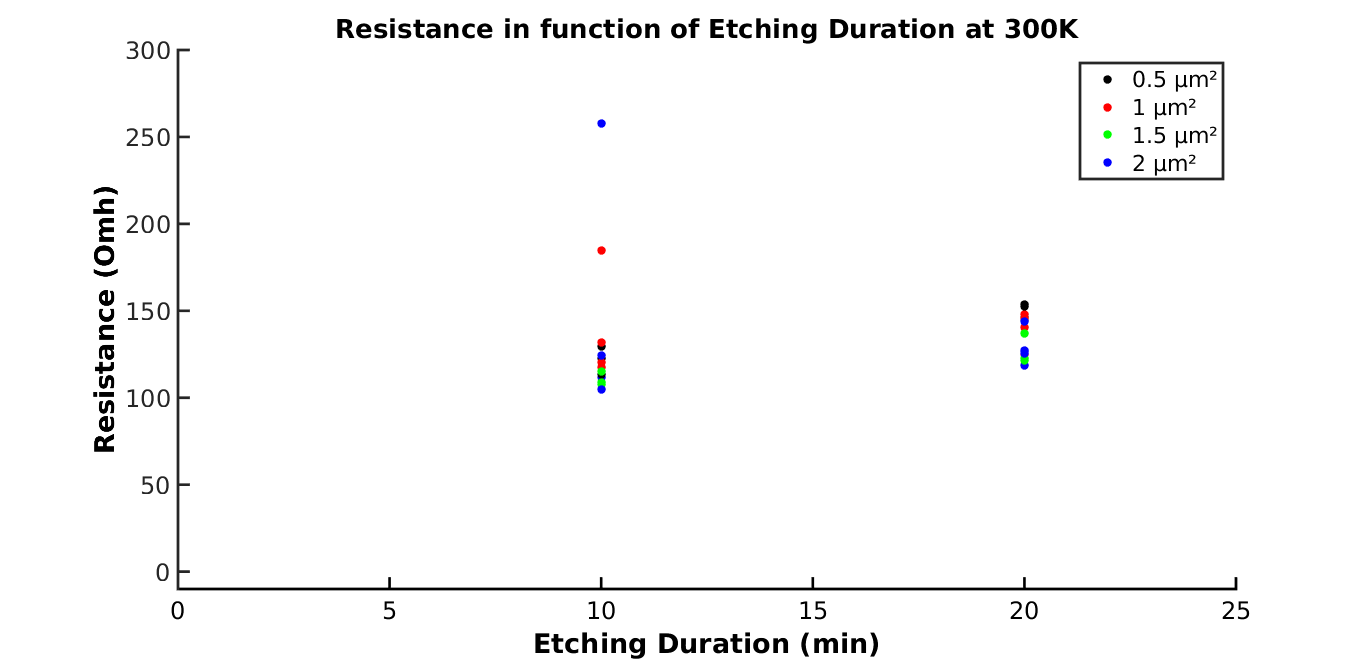
\includegraphics[width=174pt]{R_TimeBefore.png}
            \end{column}
            \begin{column}{0.5\textwidth}
                \hspace{0.5cm} $\bullet$ After Oxigen cleaning\\
                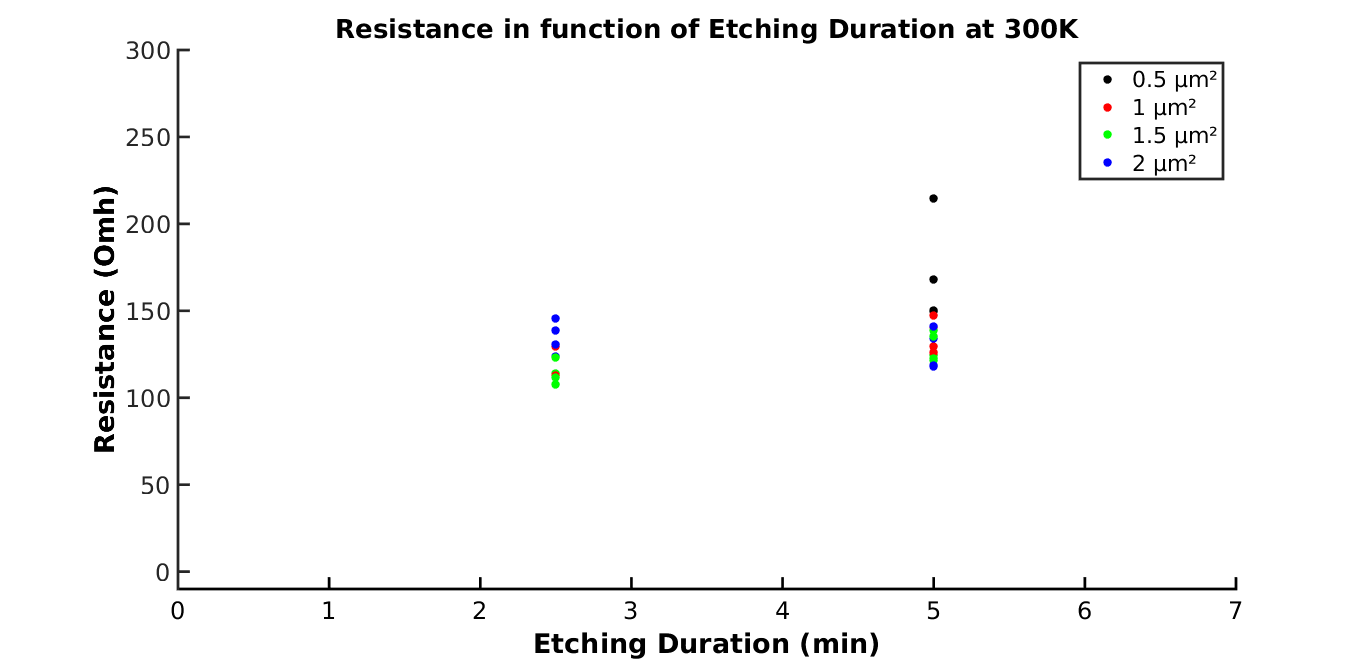
\includegraphics[width=174pt]{R_TimeAfter.png}
            \end{column}
        \end{columns}
        
        \vspace{0.5cm}
        
        $\Longrightarrow$ Similar results for totally different parameters before and after the cleaning. Before, it seems 10 min of Plasma was a good time, after the cleaning, it seems that less than 5 min is enough and that 10 min is too much.
        \vspace{2cm}
                           
        $\bullet$  Failed Samples with 10 min of Plasma and Oxidation
        \vspace{0.2cm}
        
        \begin{columns}[onlytextwidth]
            \begin{column}{0.5\textwidth}
                $\bullet$ Before Oxigen Cleaning\\
                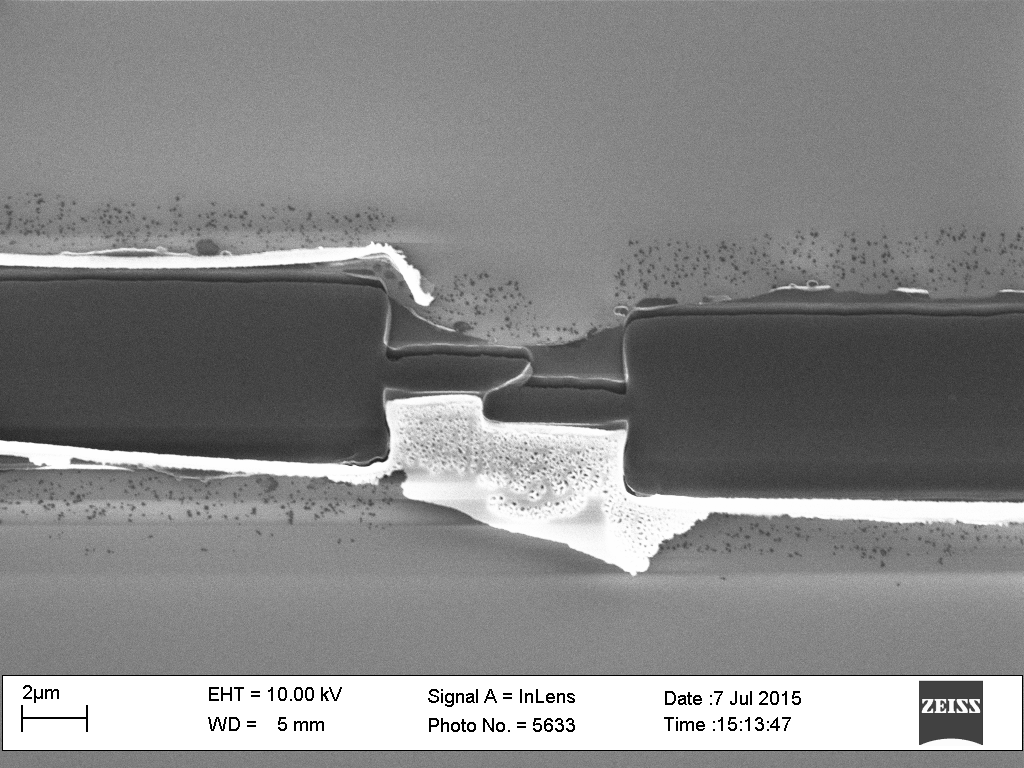
\includegraphics[width=165pt]{Burned2.png}
            \end{column}
            
            \begin{column}{0.5\textwidth}
                $\bullet$ After Oxigen cleaning\\
                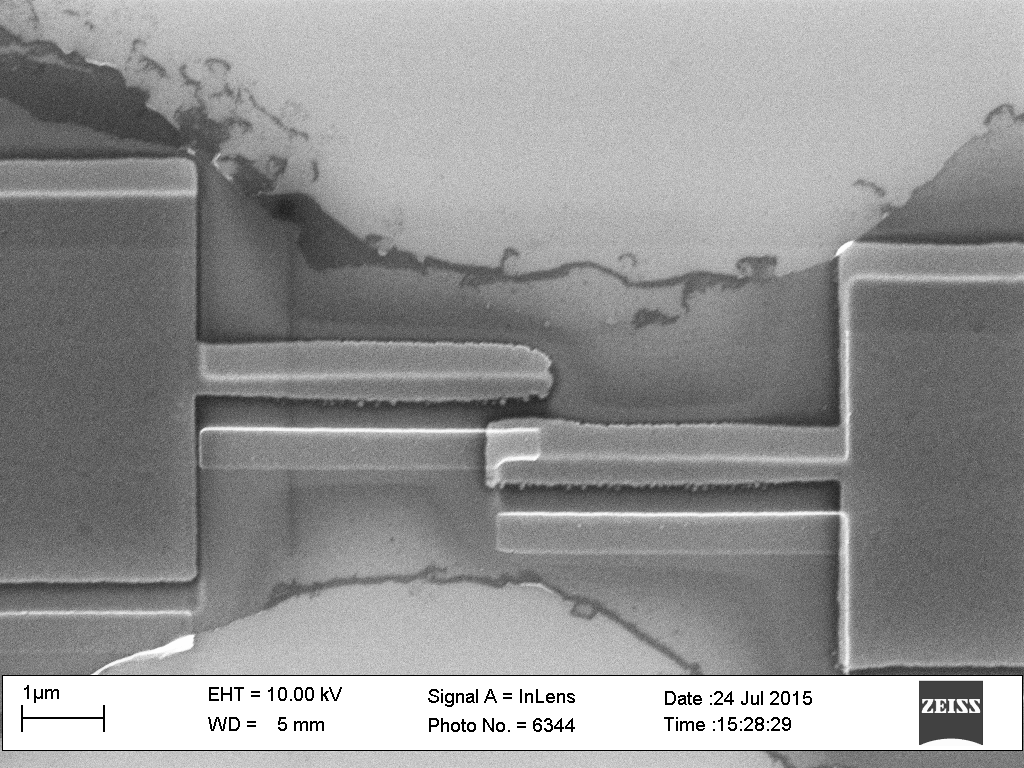
\includegraphics[width=165pt]{Burned1.png}
            \end{column}
        \end{columns}
        $\Longrightarrow$ Exact same parameters (Oxidation 10min / 200mbar, Plasma Etching 10min, Oxidation 2 min/2mbar). Before the cleaning : resist burned. After the cleaning, we do not really understand what we see.
         \vspace{2cm}
               
    $\bullet$ Wafer etching : 10 min of plasma is too much after the cleaning. Same sample as before, with a tilted angle in SEM.
       \vspace{0.5cm}
       \begin{columns}[onlytextwidth]
            \begin{column}{0.5\textwidth}
                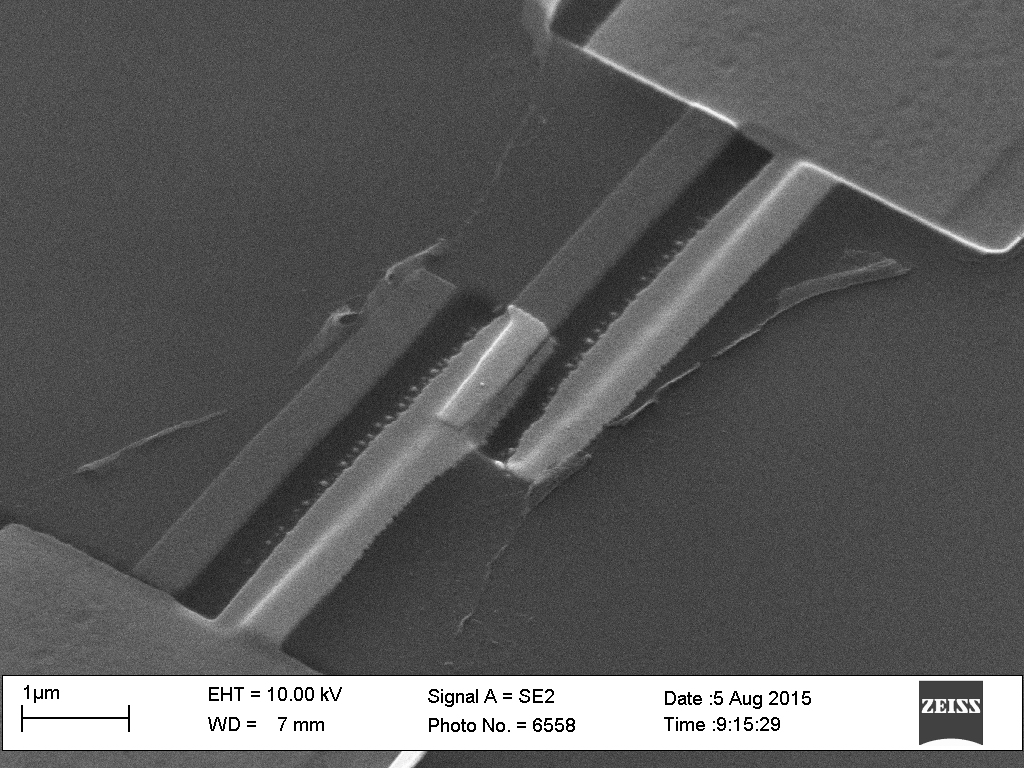
\includegraphics[width=165pt]{tilt3.png}
            \end{column}
            
            \begin{column}{0.5\textwidth}
                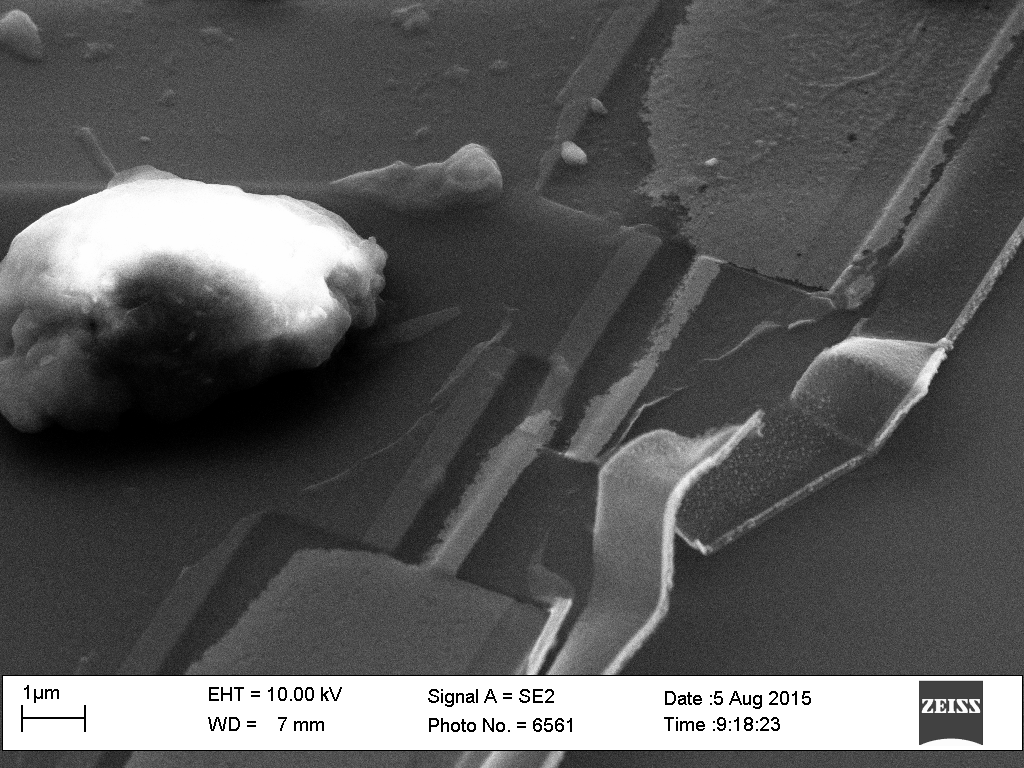
\includegraphics[width=165pt]{tilt4.png}
            \end{column}
        \end{columns}
        
       These samples had a 10k$\Omega$ resistance at room temperature, now we can understand why : there are no Al leads anymore which increase the resistance.
    \end{frame}
    
    \begin{frame}
        \frametitle{\textsc{Before the LISA maintenance}}
        \framesubtitle{Low temperature measurements}

        $\bullet$ Regular Oxidation 2min / 2mbar NIS without Plasma.\\
        \hspace{4.7cm}Leakage $\simeq$ $10^{-4}$
      
       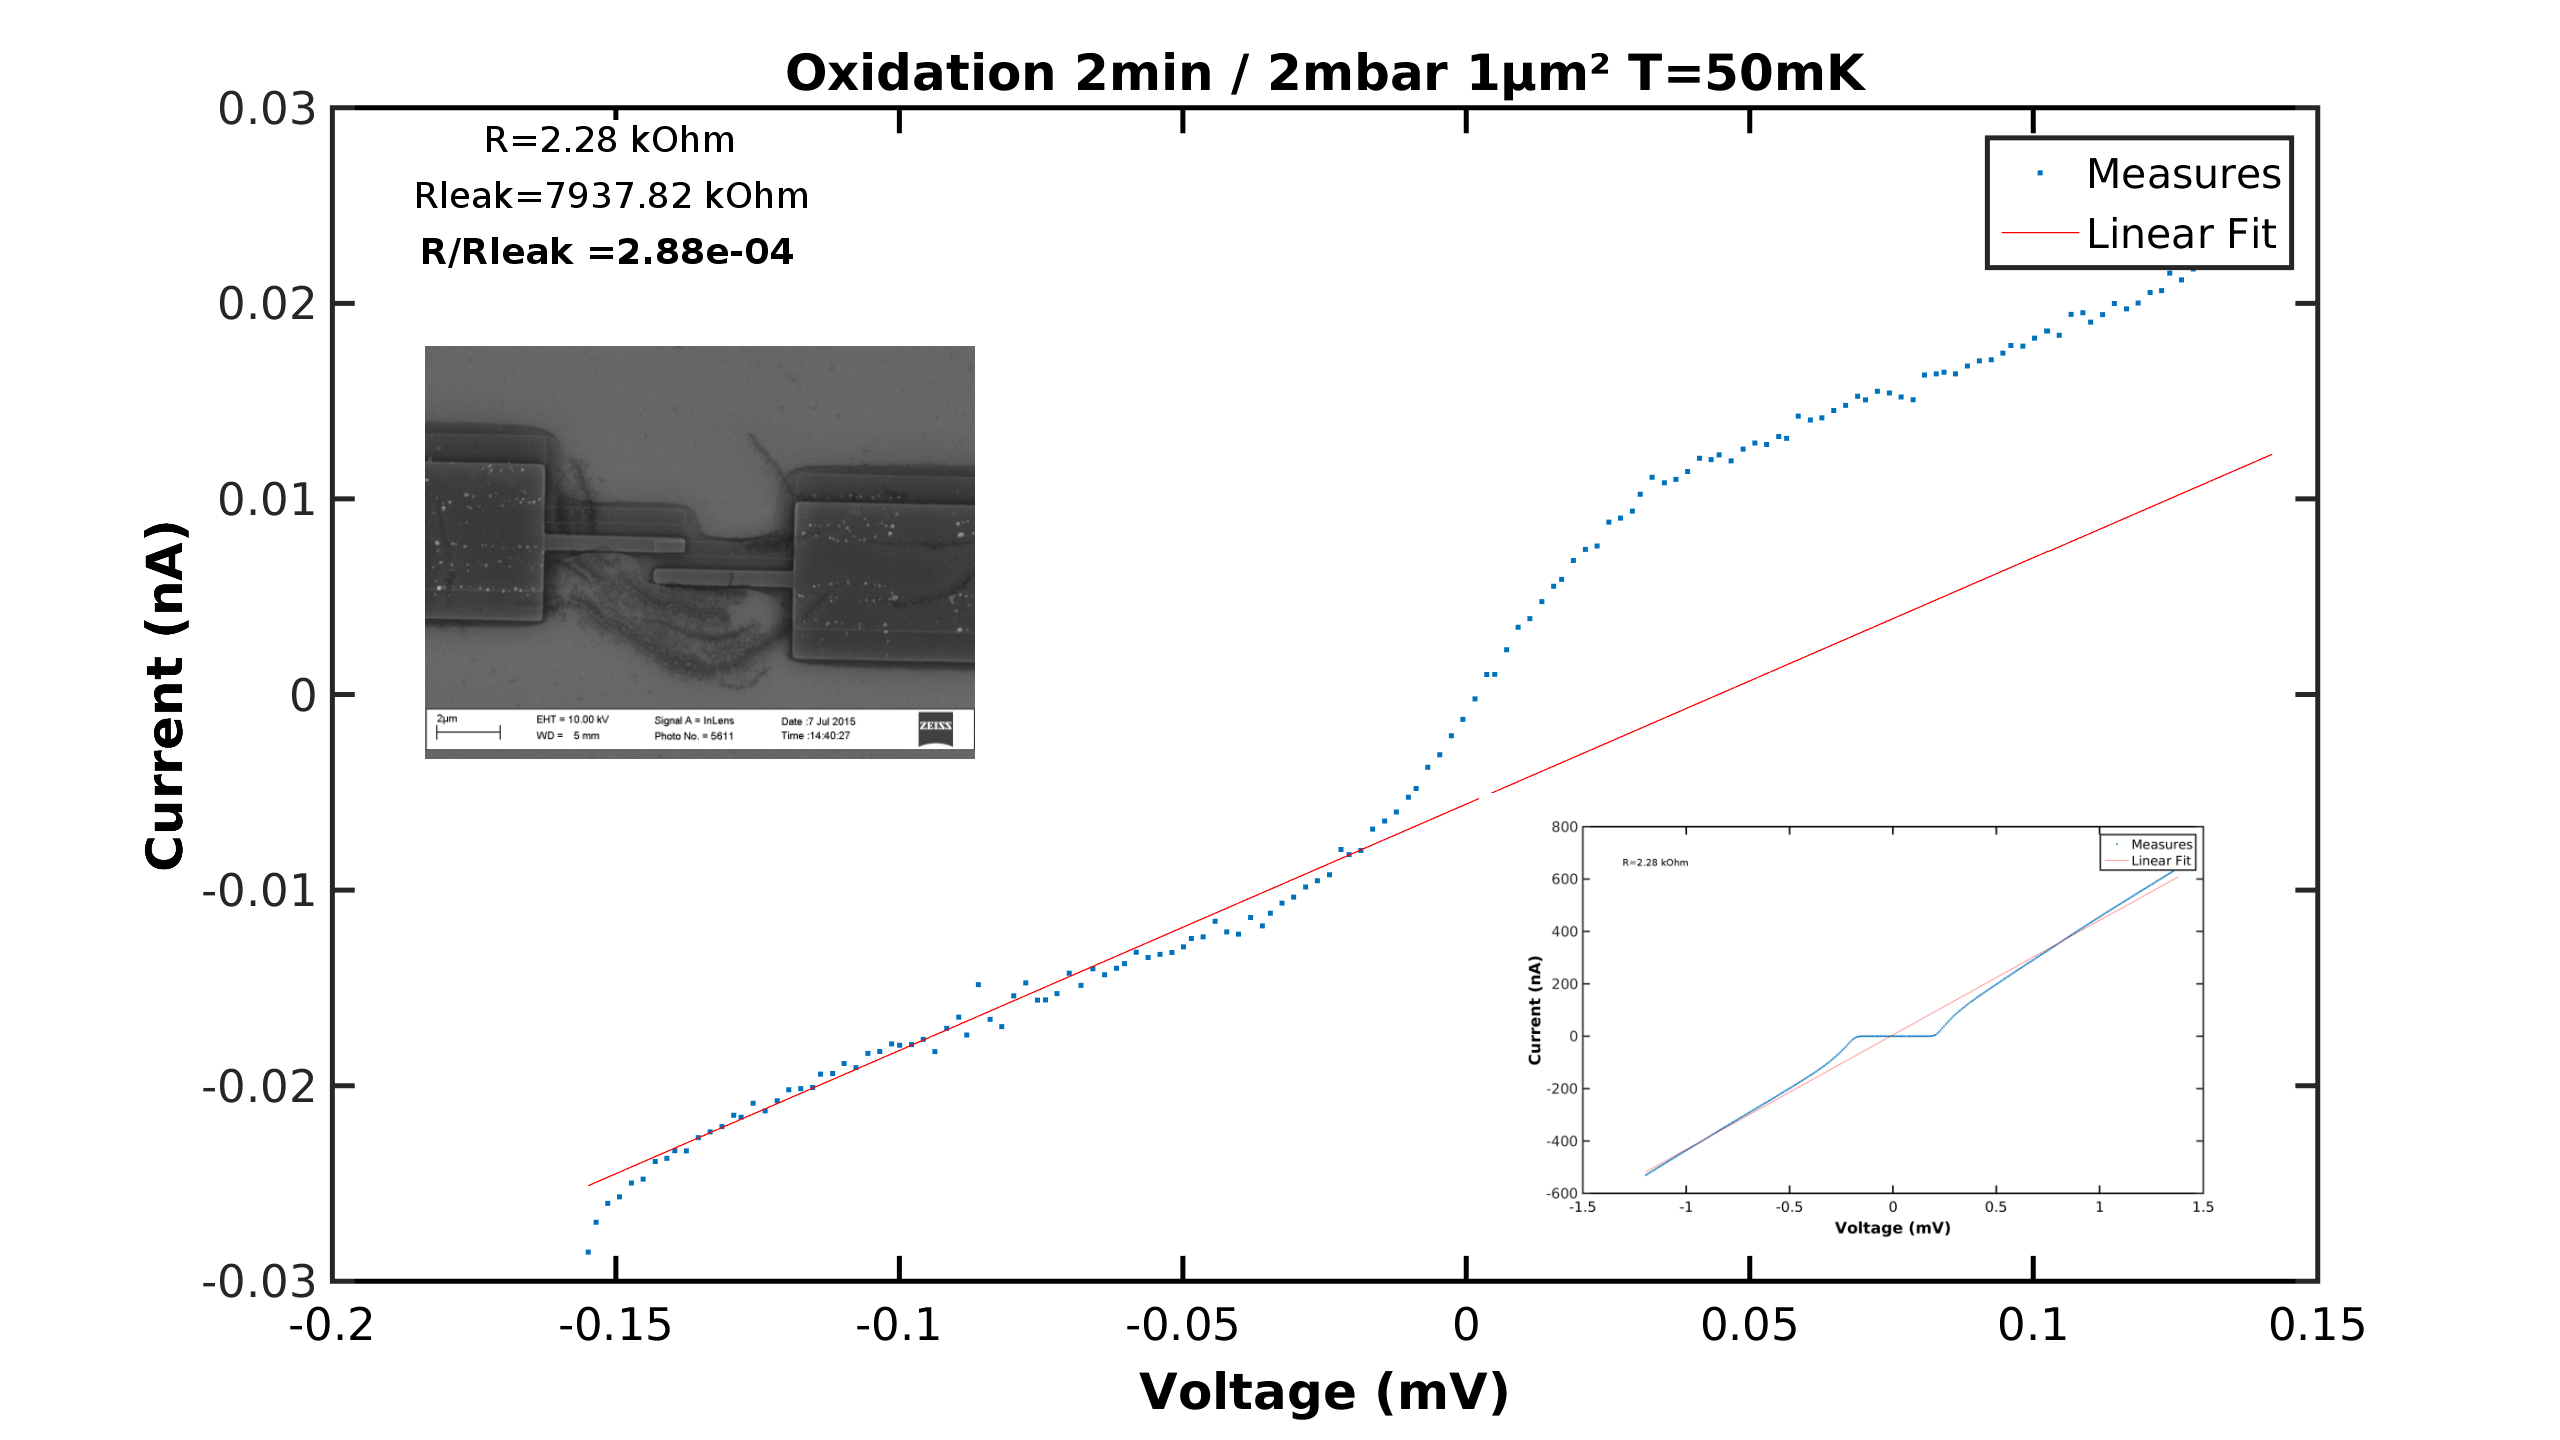
\includegraphics[width=320pt]{BeforeLISAOx.png}
        
        $\Longrightarrow$ Correct leakage.     
        
    \end{frame}
    
    \begin{frame}[allowframebreaks]
        \frametitle{\textsc{After LISA maintenance}}
        \framesubtitle{Low temperature measurements}
        
        $\bullet$  Regular Oxidation 2min / 2mbar NIS just after the maintenance without Plasma.\\
        \hspace{4.7cm} Leakage $\simeq$ $10^{-4}$
        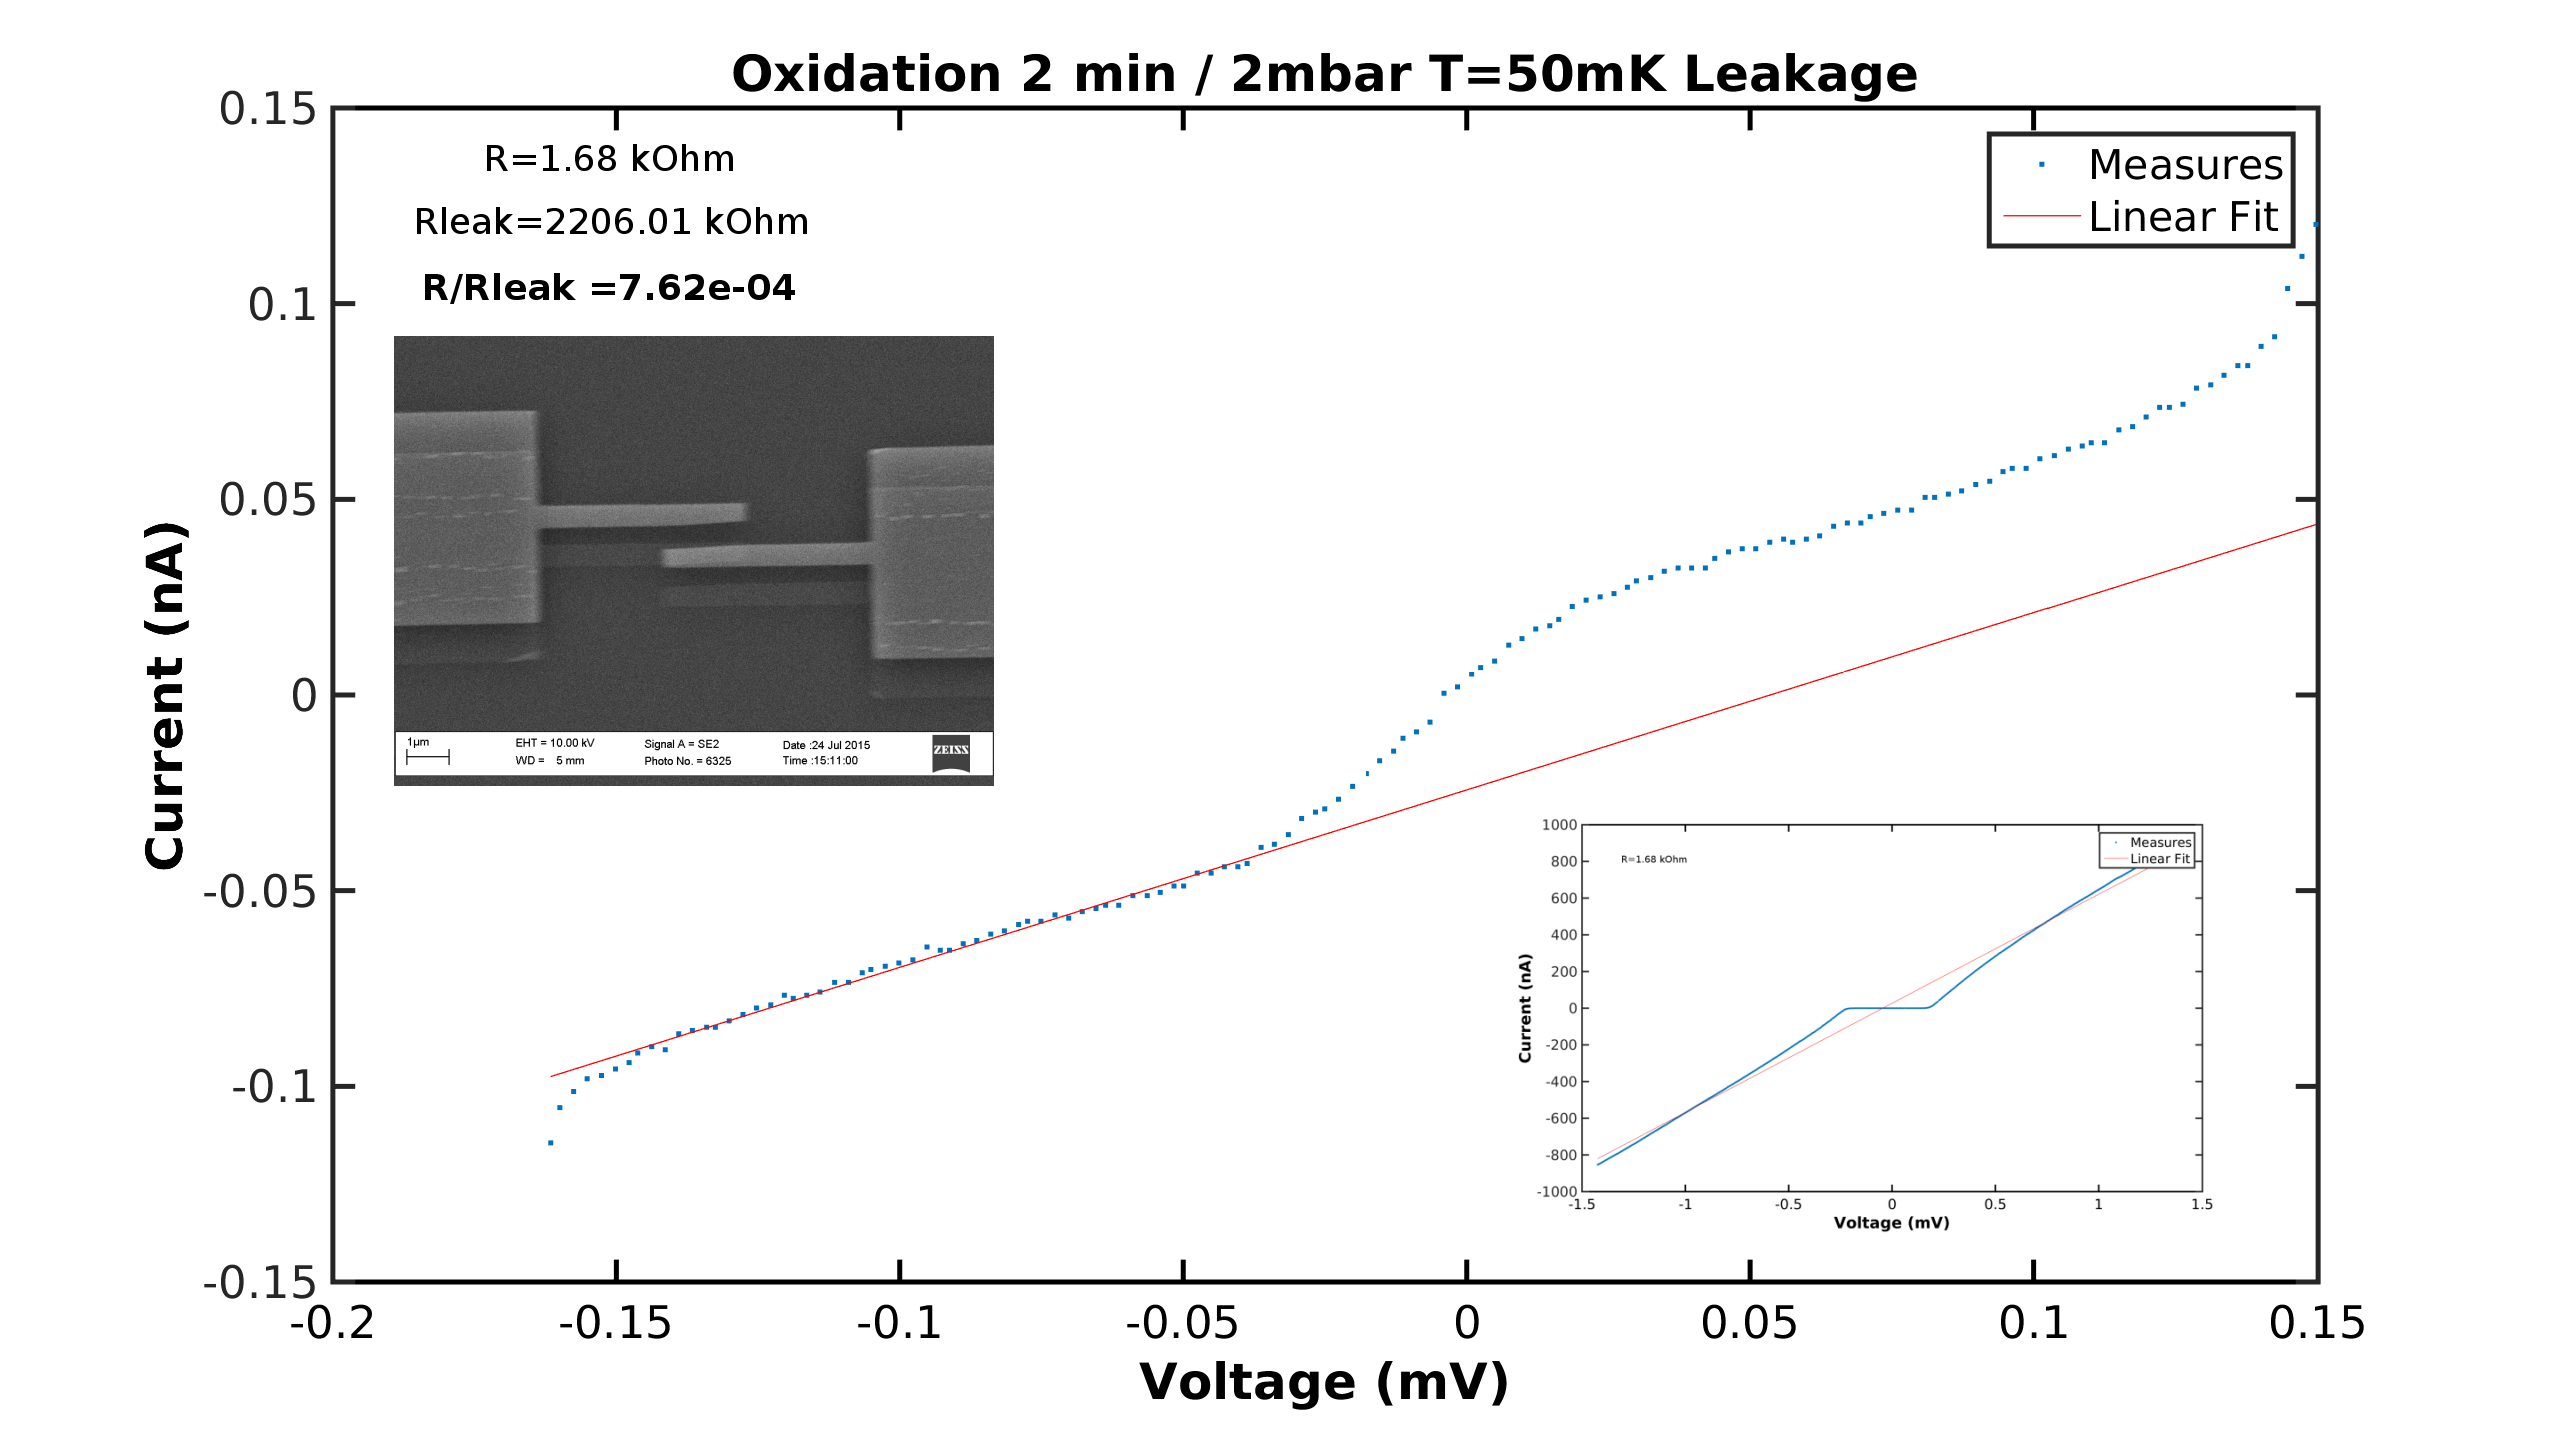
\includegraphics[width=300pt]{AfterLISAOx.png}
        \vspace{0.5cm}
        
        $\bullet$ Plasma Oxidation \hspace{1.8cm} Leakage $\simeq$ $10^{-2}$
        
        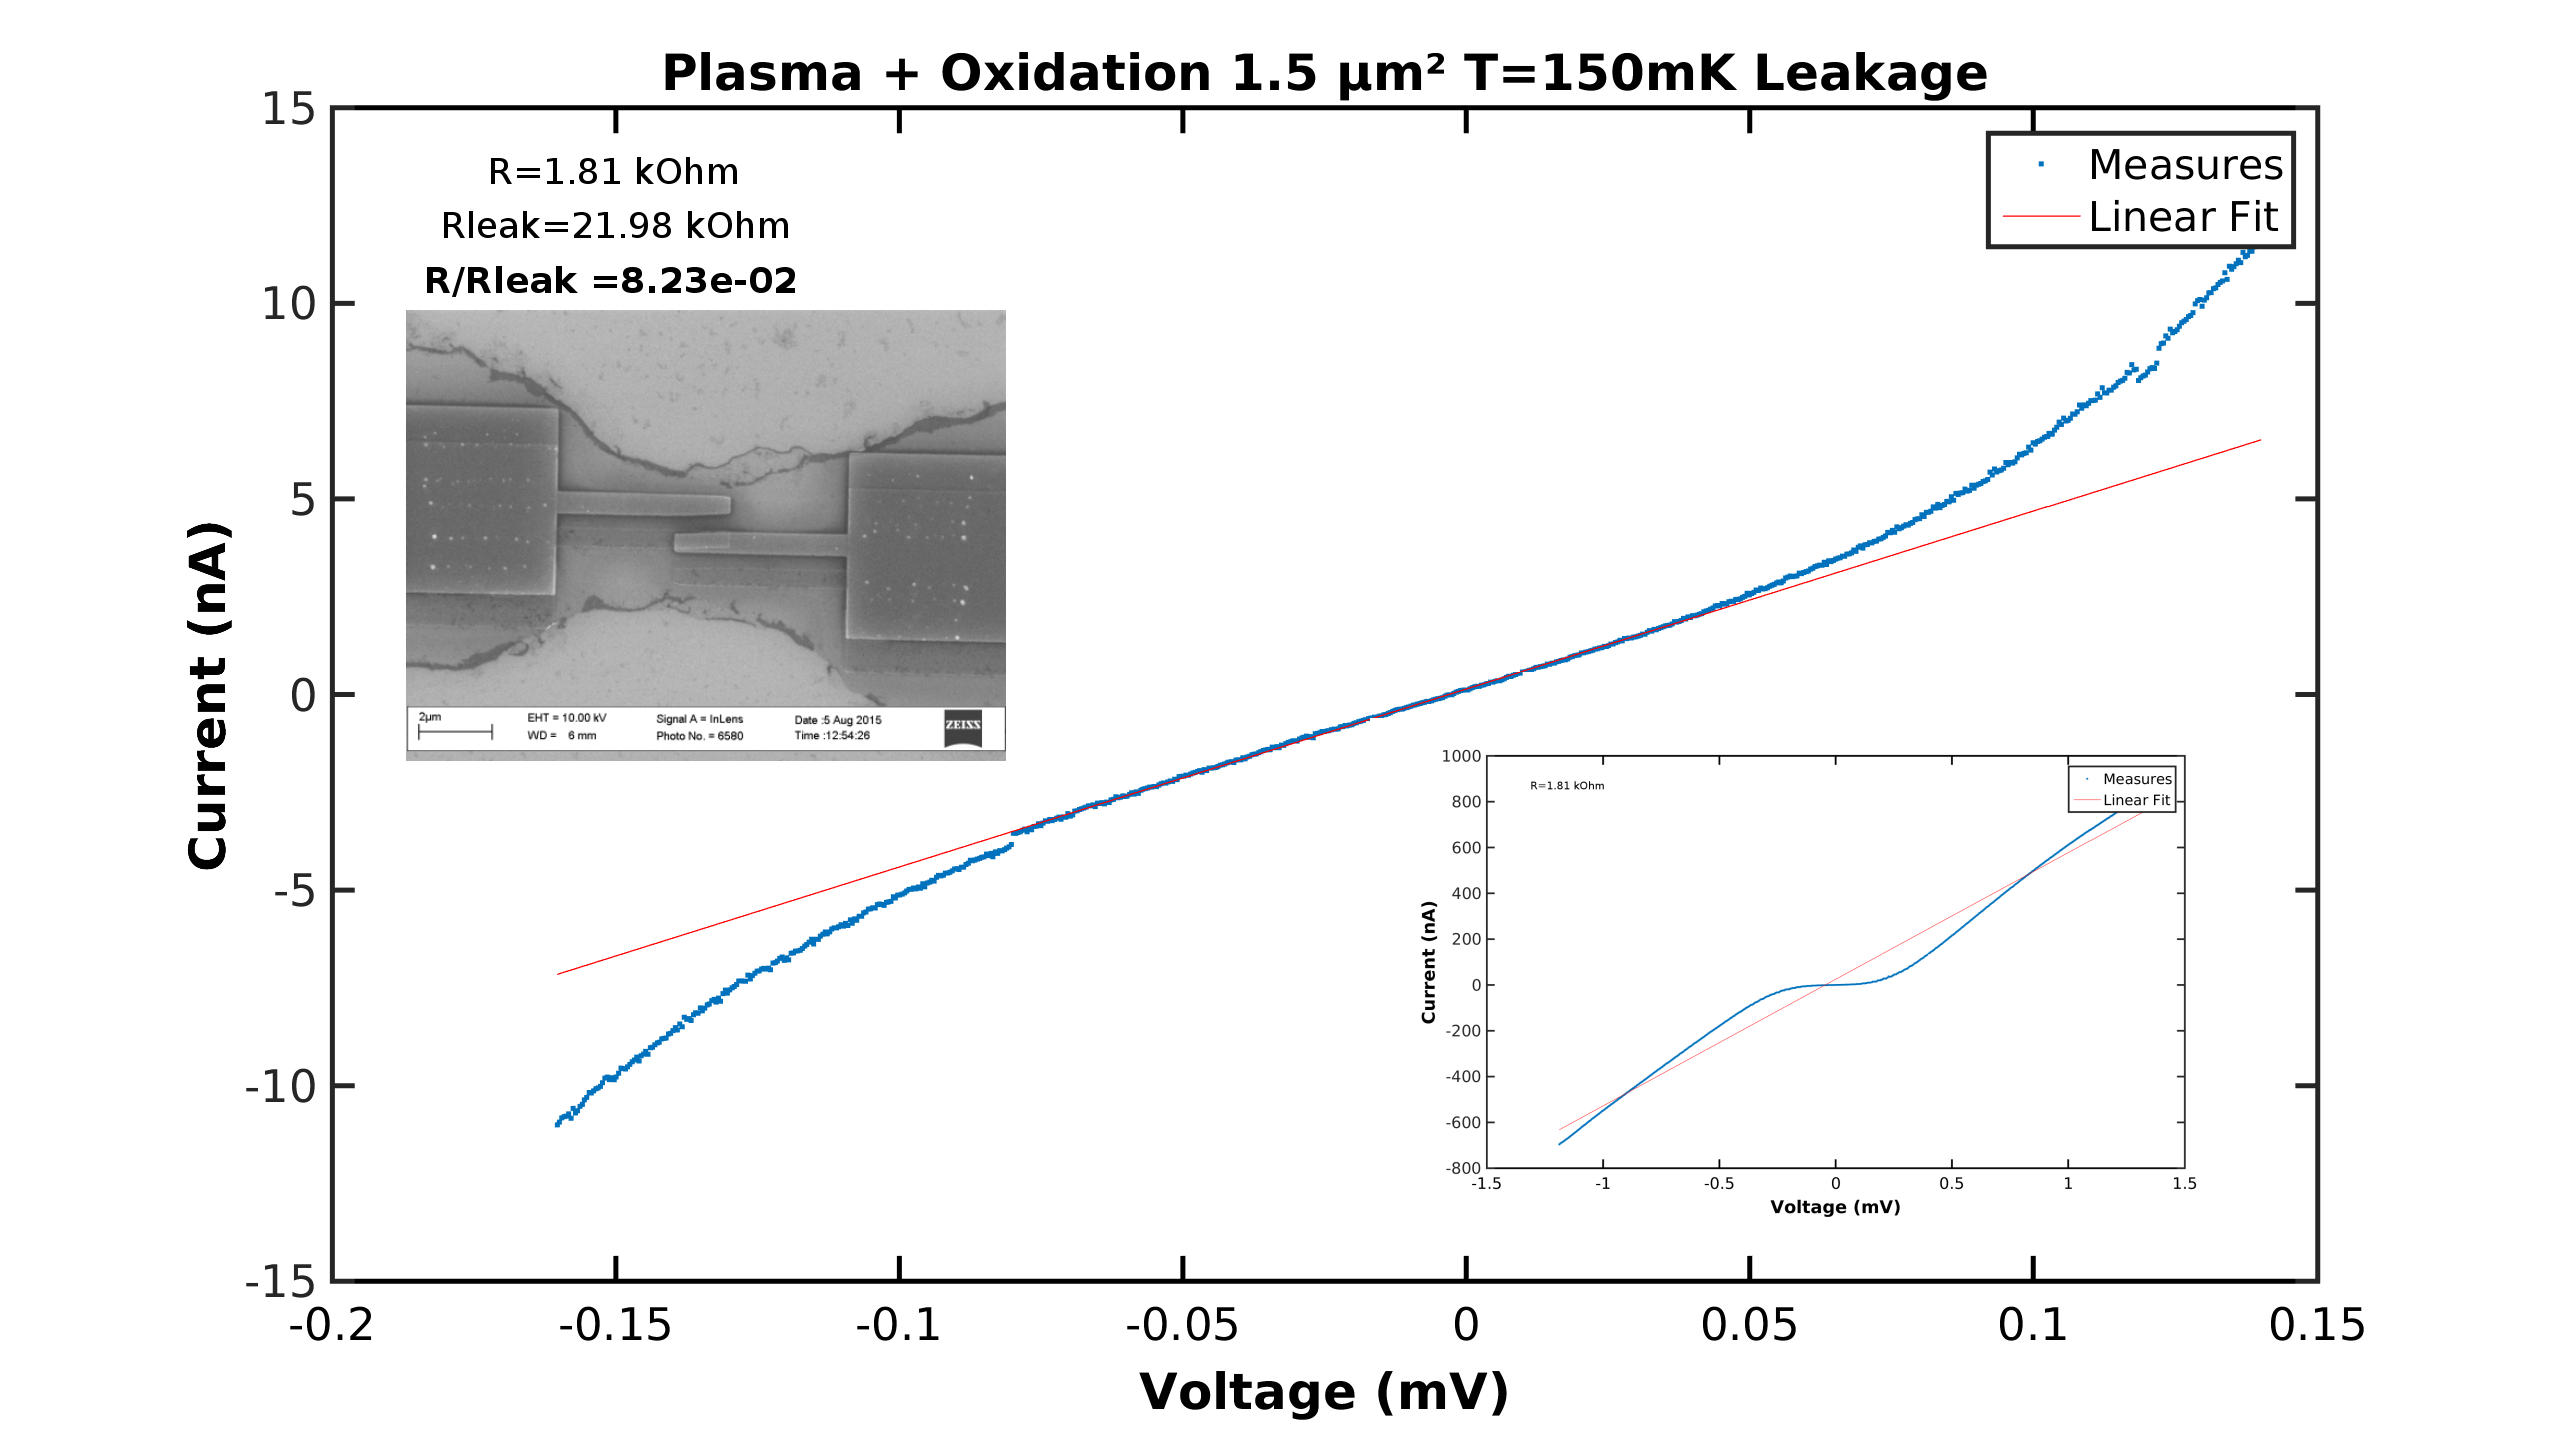
\includegraphics[width=320pt]{PlasmaOx.png}
                
        $\Longrightarrow$ The leakage is quite bad but...
        \vspace{0.5cm}
        
        $\bullet$ Regular Oxidation reference \hspace{1cm} Leakage $\simeq$ $10^{-2}$
        
        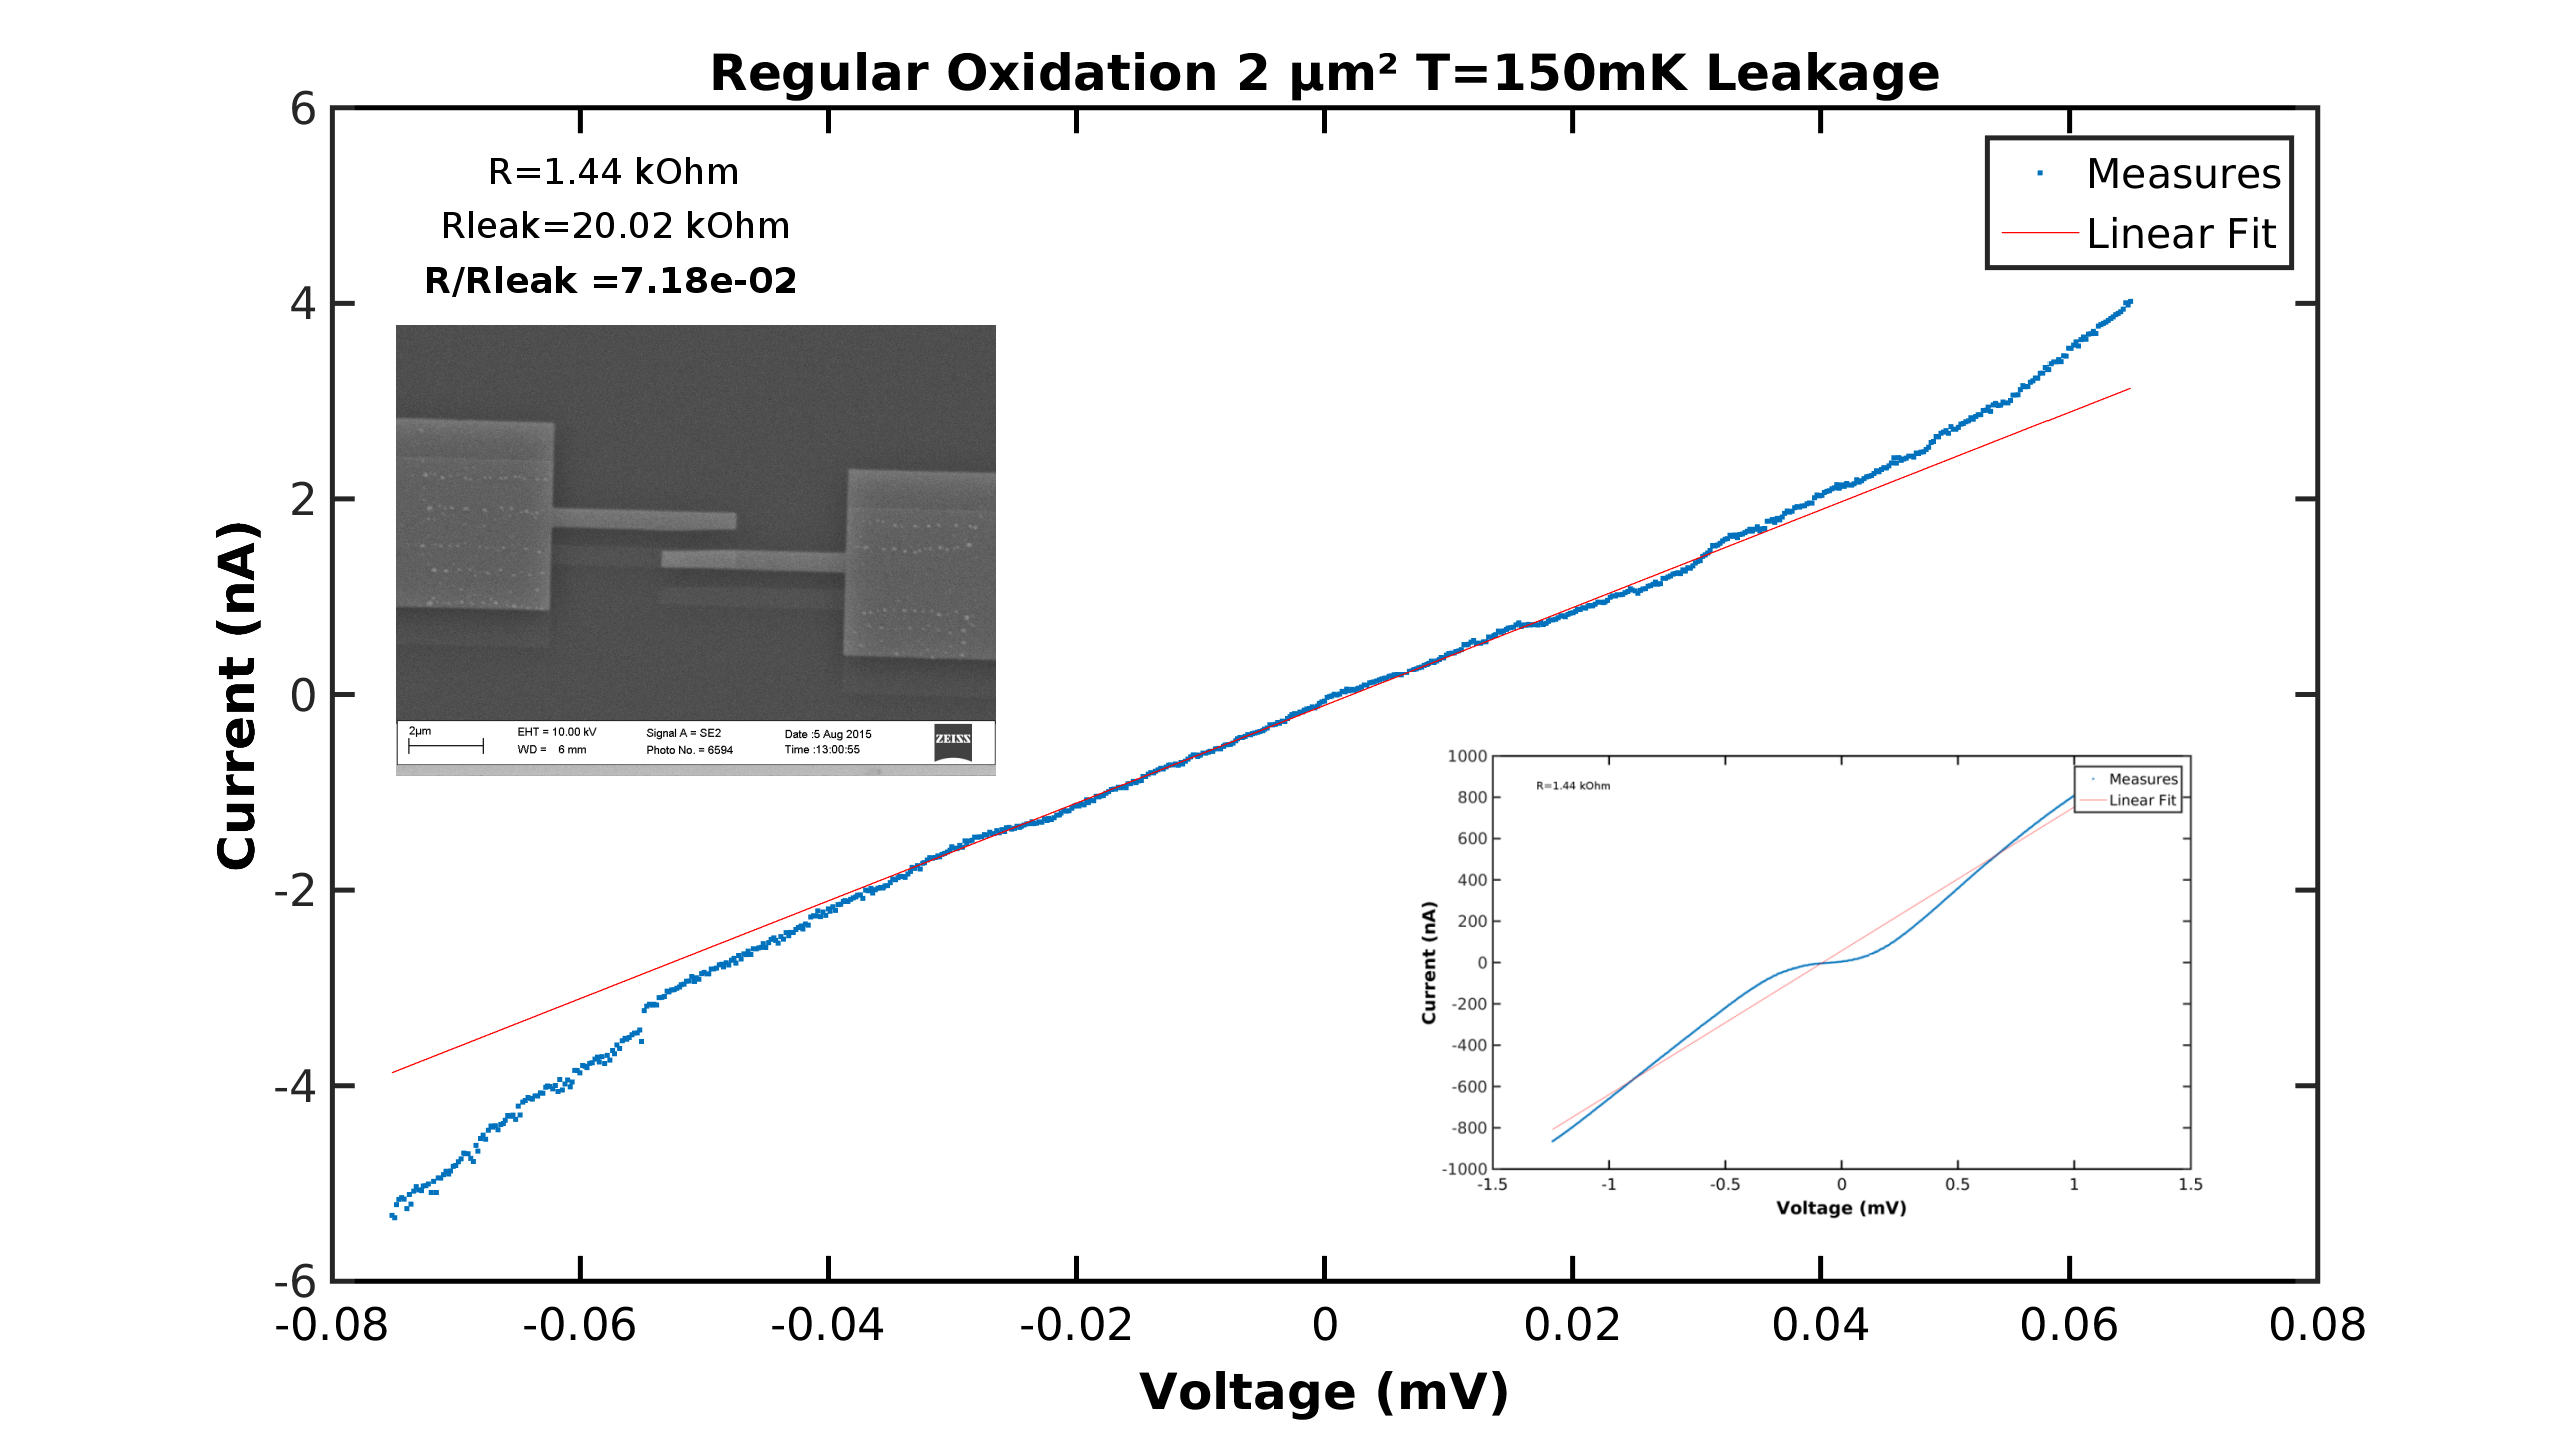
\includegraphics[width=300pt]{RegularOxRef.png}
        
        It is about the same order of magnitude for a Plasma + Oxidation sample and a Regular Oxidation Sample.

    \end{frame}
    \begin{frame}
           \frametitle{\textsc{Conclusion}}
           \framesubtitle{Summary}
           \begin{itemize}
               \item Before the cleaning, when the plasma worked well : 10 min were good to etch Al Oxide created by 10 min / 200mbar of $O_2$, the samples without Plasma had a good leakage ($10^{-4}$).
               \item The Plasma started to have problems and burned the resist of several samples, samples without Plasma remained good.
               \item The Plasma gun was cleaned, the parameters changed : 5 min were enough to etch Al Oxide created by 10 min / 200mbar of $O_2$, 10 min of Plasma etched the wafer, the samples without plasma still had a good leakage ($10^{-4}$).
               \item The leakage of all the junctions started to be poor ($10^{-2}$).
               \item Hoping that this week end maintenance will fix it up.
           \end{itemize}
           
    \end{frame}
    \begin{frame}
        \frametitle{\textsc{Conclusion}}
        \begin{LARGE}
        
        \centering    
        \textbf{Thank you for your attention !}
        \vspace{0.5cm}
        
        \textbf{If you have any questions please ask.}
        
        \end{LARGE}

       \end{frame}
       
      
    \end{document}
